\chapter{电流–电势曲线}\label{ch:b2:current-potential-curves}

锌可以从酸性镀液中电镀到钢上。然而
本科一年级分册的 E–pH 图表明，锌远低于氢线，应当会还原酸，
并与沉积同时溶解。实际并非如此，因为
图只说明什么可能发生，而不说明有多快。电极反应的速率
就是电流，将该电流对电极电势作图，
便能一眼看出哪些反应快、哪些慢，哪些
受反应物供应的限制。这些电流–电势曲线是
每位电镀金属、给电池充电或测定
河水中氧含量的电化学工作者都要用的工具。

\begin{recall}
本科一年级分册：电极电势、参比电极、能斯特
方程、E–pH 图及其局限（它们说明什么是可能的，而非
反应有多快）。\cref{ch:b2:cell-thermodynamics}：$\Delta_r G = -nFE$，能斯特
方程的推导。来自物理学：扩散与菲克定律，$j = -D\,dc/dx$。
\end{recall}

\begin{omfigure}
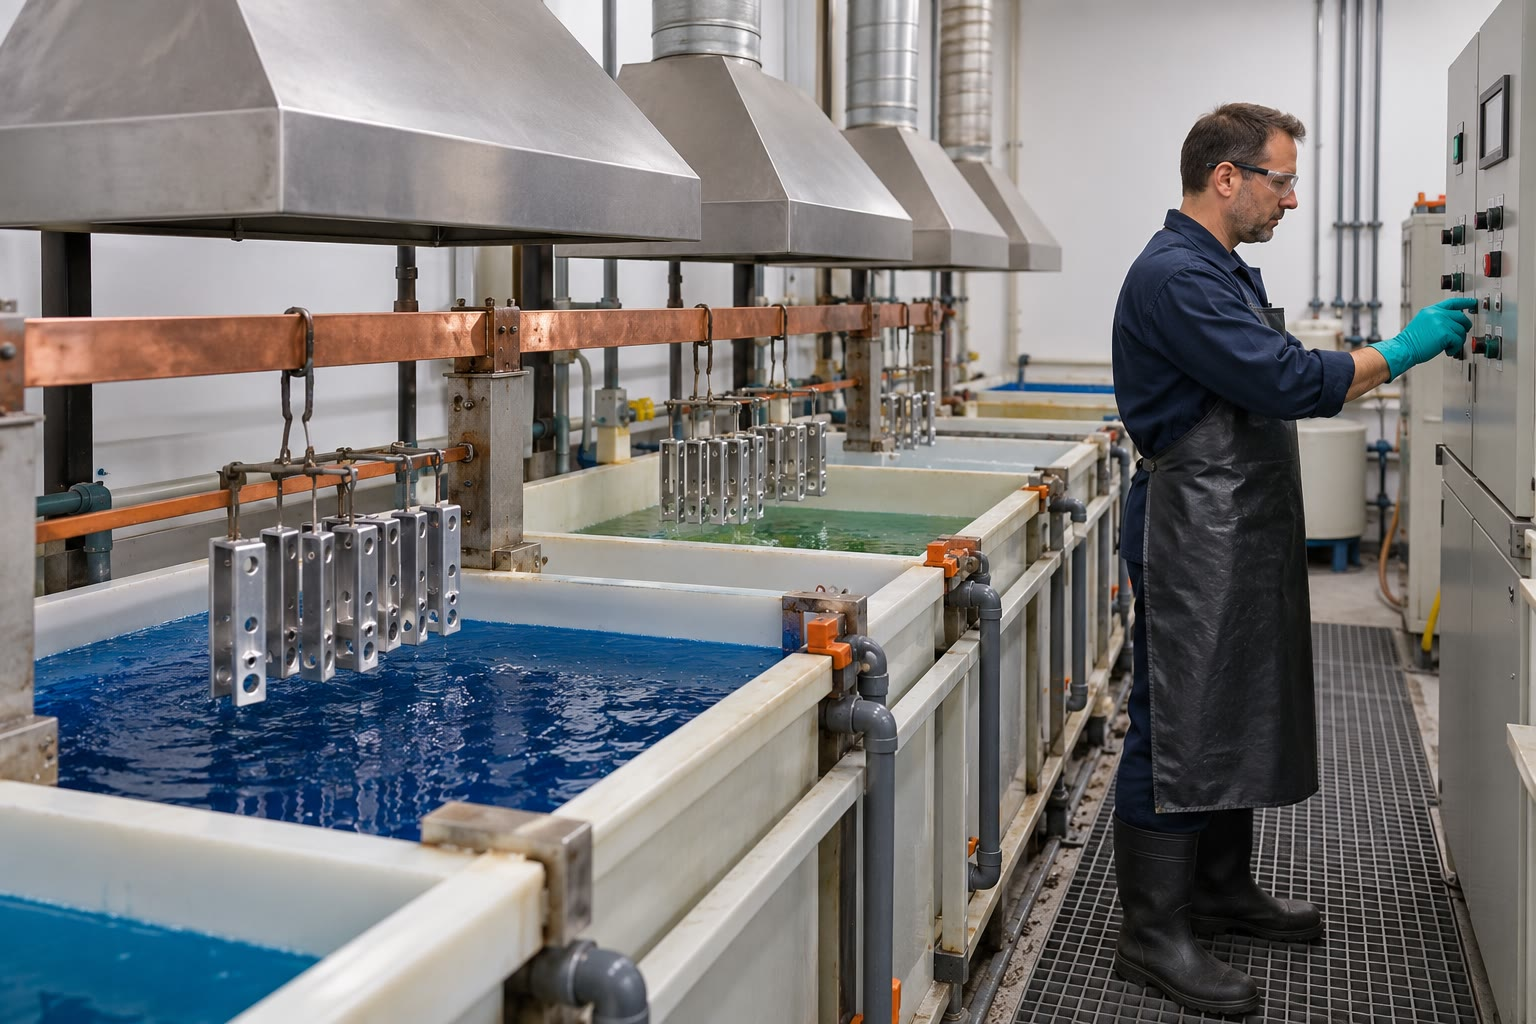
\includegraphics[width=0.62\linewidth]{images/book3/ai/b2-10-electroplating.jpg}

{\small 电镀生产线：待镀工件挂在铜母线上，
浸入镀槽并作为阴极；操作人员在整流器上设定电流。
电流决定金属沉积的快慢，工件的电势
决定沉积的是何种金属，以及与之同时析出多少氢气。}
\end{omfigure}

\section{偏离平衡的电极}

\begin{definition}[电流–电势曲线]\label{def:b2:current-potential-curves:ie-curve}
称溶液中电极的\emph{电流–电势曲线}\index{电流–电势曲线}为
流经该电极的电流 $i$ 关于
其电势 $E$ 的图像。\emph{阳极电流}\index{阳极电流}
规定为正，对应于电极上的氧化；
\emph{阴极电流}\index{阴极电流}规定为负，对应于
还原。
\end{definition}

\begin{definition}[电活性物质]\label{def:b2:current-potential-curves:electroactive}
\emph{电活性物质}\index{电活性物质}是指一类物种，
在所考虑的电势范围内能够在电极上被
氧化或还原。
\end{definition}

\begin{proposition}[电流与速率]\label{prop:b2:current-potential-curves:current-rate}
若电极上仅发生一个涉及 $n$ 个电子的半反应，则
电流度量其速率：$i = nF\,d\xi/dt$，$\xi$ 为
氧化反应的进度（因此氧化时 $i > 0$，还原时 $i < 0$）。
\end{proposition}

\begin{proof}
由\cref{prop:b2:cell-thermodynamics:charge}，进度 $d\xi$ 使
电荷 $nF\,d\xi$ 在时间 $dt$ 内流过电极。
\end{proof}

要记录此类曲线，须对一个电极施加并测量其电势，
同时使电流流过该电极——双电极电池做不到这一点，
因为电流同时也会改变第二个
电极的电势。

\begin{definition}[三电极装置]\label{def:b2:current-potential-curves:set-up}
在三电极装置中，电流在\emph{工作
电极}\index{工作电极}（所研究的电极）与\emph{对电极}\index{对电极}之间流动，
对电极用以闭合回路；工作电极的电势
以参比电极为基准测量，参比电极中
无电流通过。电子恒电势仪调节电流，
使该电势保持在设定值。
\end{definition}

\begin{omfigure}
\begin{tikzpicture}[font=\small, >={Stealth}]
  \pic[transform shape] at (0,0) {beaker={0.7}{omDef!14}};
  \pic at (-0.55,0.25) {electrode={black!35}};
  \pic at (0.55,0.25) {electrode={black!15}};
  \pic (r) at (0.0,0.15) {probe};
  \draw[thick, rounded corners] (-2.2,4.3) rectangle (2.2,5.5);
  \node at (0,4.9) {恒电势仪};
  \draw[thick, omThm] (-0.40,2.65) -- (-0.40,3.5) -- (-1.6,3.5) -- (-1.6,4.3);
  \draw[thick, omDef] (0.70,2.65) -- (0.70,3.5) -- (1.6,3.5) -- (1.6,4.3);
  \draw[thick] (r-top) -- (0,4.3);
  \node[anchor=east, font=\scriptsize, omThm] at (-1.65,3.85) {WE};
  \node[anchor=west, font=\scriptsize, omDef] at (1.65,3.85) {CE};
  \node[anchor=west, font=\scriptsize] at (0.05,3.95) {RE};
  \draw[<-, omProp, thick] (-0.75,1.2) -- (-2.0,1.4) node[left, text=black, align=right] {工作 \\ 电极};
  \draw[<-, omProp, thick] (0.85,1.2) -- (2.1,1.4) node[right, text=black, align=left] {对 \\ 电极};
  \draw[<-, omProp, thick] (0.05,0.5) -- (1.4,-0.4) node[right, text=black] {参比电极};
  \node[font=\scriptsize, align=center] at (0,6.0) {施加 $E_{\text{WE}} - E_{\text{RE}}$，测量 $i$};
\end{tikzpicture}

{\small 三电极装置。恒电势仪驱动电流
在工作电极（WE）与对电极（CE）之间流动，以
保持工作电极的电势（以参比电极为基准测得）
为设定值；参比电极（RE）中
无电流通过。}
\end{omfigure}

若无电流通过，且电对的两种形态同时存在，则电极
取该电对的能斯特电势——前提是电子交换足够快，
足以建立该电势。使电势偏离该值，便会有电流
流过。

\section{快速体系与慢速体系}

\begin{definition}[过电势]\label{def:b2:current-potential-curves:overpotential}
\emph{过电势}\index{过电势}是指流过电流
$i$ 的电极的 $\eta = E(i) - E_{\text{平衡}}$，即其
电势与该电对的平衡（能斯特）电势之差。
\emph{阈值电势}\index{阈值电势}是指一个半反应的
电势，超过它后其电流变得明显。
\end{definition}

\begin{definition}[快速体系与慢速体系]\label{def:b2:current-potential-curves:fast-slow}
某电对在给定电极上，若电势一偏离其能斯特电势，
便有明显电流流过，则称其为\emph{快速体系}\index{快速体系}；
若需要约十分之几伏的过电势，
在任一方向上电流才明显出现，则称其为
\emph{慢速体系}\index{慢速体系}。
\end{definition}

体系属于快速还是慢速，取决于电对与电极材料。
\ce{Fe^3+}/\ce{Fe^2+} 与 \ce{Ag+}/\ce{Ag} 两电对在铂上是快速的；
\ce{H+} 的还原在铂上是快速的，但在汞、铅或锌上是慢速的；
水氧化为氧气在所有电极上都是慢速的。
断裂或形成化学键的电子转移（如 \ce{O2}、\ce{H2}）通常是慢速的；
两个形状几乎相同的离子之间的电子转移则是快速的。
慢速曲线上升部分的形状来源于电子转移动力学，
该内容将在本科三年级分册中推导。

\begin{omfigure}
\begin{tikzpicture}
\begin{axis}[omie, width=0.47\linewidth, height=5.4cm, xmin=0.25, xmax=1.3,
  ymin=-1.3, ymax=1.3, xlabel={$E$}, ylabel={$i$}, title={\small 快速体系}]
\addplot[omanodic] table[x=E, y=i, restrict expr to domain={\thisrow{i}}{0:2}] {figdata/out/bachelor-2-ie-curves-a.dat};
\addplot[omcathodic] table[x=E, y=i, restrict expr to domain={\thisrow{i}}{-2:0}] {figdata/out/bachelor-2-ie-curves-a.dat};
\draw[densely dotted] (axis cs:0.77,-1.2) -- (axis cs:0.77,1.2);
\node[font=\scriptsize, anchor=north west] at (axis cs:0.78,-0.05) {$E_{\text{平衡}}$};
\node[font=\scriptsize, anchor=south] at (axis cs:1.1,1.0) {\ce{Fe^2+} $\to$ \ce{Fe^3+}};
\node[font=\scriptsize, anchor=north] at (axis cs:0.45,-1.0) {\ce{Fe^3+} $\to$ \ce{Fe^2+}};
\end{axis}
\end{tikzpicture}\hfill
\begin{tikzpicture}
\begin{axis}[omie, width=0.47\linewidth, height=5.4cm, xmin=-0.25, xmax=1.8,
  ymin=-1.3, ymax=1.3, xlabel={$E$}, ylabel={$i$}, title={\small 慢速体系}]
\addplot[omanodic] table[x=E, y=i, restrict expr to domain={\thisrow{i}}{0:2}] {figdata/out/bachelor-2-ie-curves-c.dat};
\addplot[omcathodic] table[x=E, y=i, restrict expr to domain={\thisrow{i}}{-2:0}] {figdata/out/bachelor-2-ie-curves-c.dat};
\draw[densely dotted] (axis cs:0.77,-1.2) -- (axis cs:0.77,1.2);
\draw[<->, omProp] (axis cs:0.77,0.5) -- (axis cs:1.12,0.5) node[midway, above, font=\scriptsize] {$\eta_a$};
\draw[<->, omProp] (axis cs:0.42,-0.5) -- (axis cs:0.77,-0.5) node[midway, below, font=\scriptsize] {$\eta_c$};
\node[font=\scriptsize, anchor=north west] at (axis cs:0.78,-0.05) {$E_{\text{平衡}}$};
\end{axis}
\end{tikzpicture}

{\small 两种形式浓度相等的某电对的模型电流–电势曲线
（阳极支为红色，阴极支为蓝色）。左图为快速体系：
电流在平衡电势附近急剧变号。右图为慢速体系：
其附近一定电势范围内无电流流过，
每一支都需要过电势。两者最终都趋于相同的极限平台，
由扩散决定。（数值仅作示意。）}
\end{omfigure}

\section{传质与极限电流}

当电子转移很快时，电流受限于
反应物到达电极的速率。在搅拌的溶液中，
紧邻电极的一薄层液体几乎静止，
反应物通过扩散穿过该层。

\begin{definition}[扩散层与极限电流]\label{def:b2:current-potential-curves:limiting-current}
电极附近溶液中的一层，厚度为 $\delta$
（搅拌溶液中约为几微米到几十微米），紧邻电极，
称为\emph{扩散层}\index{扩散层}，其中物质仅通过扩散移动。
当电活性物质到达电极后被立即消耗、
其表面浓度为零时所达到的电流，称为
\emph{极限电流}\index{极限电流}。
\end{definition}

\begin{omfigure}
\begin{tikzpicture}[font=\small, >={Stealth}, x=1.2cm, y=1.2cm]
  \fill[black!25] (-0.4,0) rectangle (0,3);
  \node[rotate=90, font=\scriptsize] at (-0.2,1.5) {电极};
  \draw[->] (0,0) -- (4.6,0) node[right] {$x$};
  \draw[->] (0,0) -- (0,3.2) node[above] {$c$};
  \draw[densely dashed] (1.6,0) -- (1.6,3);
  \node[below, font=\scriptsize] at (1.6,0) {$\delta$};
  \draw[omDef, thick] (0,1.2) -- (1.6,2.4) -- (4.4,2.4);
  \draw[omThm, thick] (0,0.02) -- (1.6,2.4);
  \node[font=\scriptsize, anchor=west] at (2.6,2.6) {本体，$c^b$（搅拌）};
  \node[font=\scriptsize, omDef, anchor=east] at (-0.45,1.2) {$c^s$};
  \node[font=\scriptsize, omThm, anchor=west] at (1.7,0.5) {$c^s = 0$：极限电流};
  \node[font=\scriptsize, align=center] at (0.8,3.0) {扩散 \\ 层};
\end{tikzpicture}

{\small 搅拌溶液中电极附近反应物的浓度。在扩散层内浓度分布为线性；
通量，进而电流，与 $c^b - c^s$ 成正比。
反应物一到达即被消耗（$c^s = 0$，红色）时，
通量最大。}
\end{omfigure}

\begin{theorem}[极限电流]\label{thm:b2:current-potential-curves:limiting}
对于本体浓度为 $c$、扩散系数为 $D$ 的物种，
穿过厚度为 $\delta$ 的扩散层、到达面积为 $A$ 的电极时，
极限电流的绝对值为
\[
  |i_{\lim}| = \frac{nFADc}{\delta} .
\]
\end{theorem}

\begin{proof}
稳态时，层内浓度分布为线性（菲克第二定律
取 $\partial c/\partial t = 0$ 得 $d^2c/dx^2 = 0$），因此朝向电极的通量为
$j = D(c - c^s)/\delta$，单位面积、单位时间的摩尔数。
每个到达的分子与 $n$ 个电子反应：$|i| = nFAj =
nFAD(c - c^s)/\delta$，当 $c^s = 0$ 时最大。
\end{proof}

\begin{example}[极限电流的大小]\label{ex:b2:current-potential-curves:ilim}
对于浓度为 \qty{10}{mmol/L}（\qty{10}{mol/m^3}）的某物种，取 $D =
\qty{7e-10}{m^2/s}$、$\delta = \qty{20}{\micro m}$、$n = 1$，电极面积为
\qty{1.0}{cm^2}：$|i_{\lim}| = 96\,485 \times 10^{-4} \times 7 \times 10^{-10}
\times 10/(2 \times 10^{-5}) = \qty{3.4}{mA}$。
\end{example}

\begin{theorem}[快速体系的波]\label{thm:b2:current-potential-curves:wave}
对于快速电对 $\mathrm{Ox} + n\,\mathrm e^- \rightleftharpoons \mathrm{Red}$，
阳极极限电流 $i_{\lim,a} > 0$（由 Red 决定）与阴极
极限电流 $i_{\lim,c} < 0$（由 Ox 决定），稳态曲线为
\[
  E = E_{1/2} + \frac{RT}{nF}\ln\frac{i - i_{\lim,c}}{i_{\lim,a} - i},
  \qquad E_{1/2} = E^\circ + \frac{RT}{nF}\ln\frac{D_{\text{Red}}}{D_{\text{Ox}}} ,
\]
两种形式的扩散层厚度相同。
\end{theorem}

\begin{proof}
快速体系：表面处满足能斯特方程 $E = E^\circ + (RT/nF)
\ln(c^s_{\text{Ox}}/c^s_{\text{Red}})$。线性分布：阳极电流 $i$
在表面消耗 Red 并生成 Ox，$i = nFAD_{\text{Red}}(c^b_{\text{Red}}
- c^s_{\text{Red}})/\delta = -nFAD_{\text{Ox}}(c^b_{\text{Ox}} - c^s_{\text{Ox}})/\delta$。
由 $i_{\lim,a} = nFAD_{\text{Red}}c^b_{\text{Red}}/\delta$ 与 $i_{\lim,c} =
-nFAD_{\text{Ox}}c^b_{\text{Ox}}/\delta$，可得 $c^s_{\text{Red}} = (i_{\lim,a} -
i)\delta/(nFAD_{\text{Red}})$，$c^s_{\text{Ox}} = (i - i_{\lim,c})\delta/(nFAD_{\text{Ox}})$。
代入能斯特方程即得。
\end{proof}

\begin{corollary}[半波电势]\label{cor:b2:current-potential-curves:half-wave}
当两种形式的扩散系数相等时，$E_{1/2} = E^\circ$：若仅存在一种形式，
则在该电对的标准电势处，电流为其极限值的
一半。
\end{corollary}

\begin{proof}
仅存在 Red 时，$i_{\lim,c} = 0$，对于 $i = i_{\lim,a}/2$，对数项
为零：$E = E_{1/2} = E^\circ$，当 $D_{\text{Red}} = D_{\text{Ox}}$ 时。
\end{proof}

\begin{proposition}[平台高度测量浓度]\label{prop:b2:current-potential-curves:plateau}
在搅拌与电极固定时，平台的高度与其所消耗的
物种的浓度成正比：将电极保持在平台上的某一
电势处，即构成安培式传感器。
\end{proposition}

\begin{proof}
$|i_{\lim}| = (nFAD/\delta)\,c$，括号内的因子在
搅拌与温度固定时为常数。
\end{proof}

\begin{omfigure}
\begin{tikzpicture}
\begin{axis}[omie, width=0.47\linewidth, height=5.0cm, xmin=0.25, xmax=1.3,
  ymin=-0.3, ymax=1.3, xlabel={$E$}, ylabel={$i$}, title={\small 仅存在 \ce{Fe^2+}}]
\addplot[omanodic] table[x=E, y=i] {figdata/out/bachelor-2-ie-curves-b.dat};
\draw[densely dotted] (axis cs:0.77,0) -- (axis cs:0.77,0.5) -- (axis cs:0.25,0.5);
\node[font=\scriptsize, anchor=north] at (axis cs:0.77,-0.02) {$E_{1/2}$};
\node[font=\scriptsize, anchor=south west] at (axis cs:0.27,0.5) {$i_{\lim}/2$};
\node[font=\scriptsize, anchor=south] at (axis cs:1.12,1.0) {平台};
\end{axis}
\end{tikzpicture}\hfill
\begin{tikzpicture}
\begin{axis}[width=0.42\linewidth, height=5.0cm, xmin=0, xmax=1.05, ymin=0, ymax=1.1,
  axis x line=bottom, axis y line=left, xtick=\empty, ytick=\empty,
  xlabel={$c$}, ylabel={$i_{\lim}$}, label style={font=\small},
  title={\small 安培法}]
\addplot[omanodic, mark=*, mark size=1.2pt] table[x=c, y=i] {figdata/out/bachelor-2-ie-curves-e.dat};
\end{axis}
\end{tikzpicture}

{\small 左：仅存在还原态时快速电对的波（模型）；
其半高位于半波电势处。右：平台高度
与浓度成正比增长。}
\end{omfigure}

\section{溶剂与电极}

水本身具有电活性：它被氧化为氧气
（\ce{2H2O -> O2 + 4H+ + 4e-}），也被还原为氢气（\ce{2H+ + 2e- -> H2}，或
\ce{2H2O + 2e- -> H2 + 2OH-}）。由于溶剂从不耗尽，其曲线
没有平台：它们急剧上升，并限定其余所有曲线的范围。

\begin{definition}[电活性窗口]\label{def:b2:current-potential-curves:window}
\emph{溶剂壁垒}\index{溶剂壁垒}是溶剂氧化与还原的
陡峭分支。\emph{电活性窗口}\index{电活性窗口}是两者之间的
电势范围，在此范围内可以观察到
溶解物种的曲线。
\end{definition}

\begin{proposition}[水的窗口]\label{prop:b2:current-potential-curves:window}
在给定 pH 的水中，窗口大致位于水的两个电对的热力学范围附近，
即 $\qty{0}{V} - 0.059\,\mathrm{pH}$ 与 $\qty{1.23}{V} -
0.059\,\mathrm{pH}$，在两侧各由所用电极上相应反应的
过电势展宽。
\end{proposition}

\begin{proof}[论证]
每一壁垒都始于其电对的能斯特电势再加上
阈值过电势的位置：水的氧化在所有电极上都很慢，因此
阳极壁垒位于 \qty{1.23}{V}（pH 0 时）之上若干十分之一伏处；
\ce{H+} 的还原在铂上很快，其阴极壁垒接近
\qty{0}{V}，但在锌、铅或汞上很慢，其壁垒则
低几十分之一伏。
\end{proof}

\begin{omfigure}
\begin{tikzpicture}
\begin{axis}[omie, width=0.82\linewidth, height=5.4cm, xmin=-1.2, xmax=2.0,
  ymin=-3, ymax=3, xlabel={$E$ (V)}, ylabel={$i$}, clip=true, clip mode=individual]
\addplot[omwall] table[x=E, y=i] {figdata/out/bachelor-2-ie-curves-d-high.dat};
\addplot[omcathodic] table[x=E, y=i, restrict expr to domain={\thisrow{E}}{-1.2:0.6}] {figdata/out/bachelor-2-ie-curves-d-Pt.dat};
\addplot[omanodic] table[x=E, y=i, restrict expr to domain={\thisrow{E}}{0.6:2.0}] {figdata/out/bachelor-2-ie-curves-d-Pt.dat};
\draw[densely dotted] (axis cs:0,-2.8) -- (axis cs:0,2.8);
\draw[densely dotted] (axis cs:1.23,-2.8) -- (axis cs:1.23,2.8);
\node[font=\scriptsize, anchor=north west] at (axis cs:0.02,-0.1) {0};
\node[font=\scriptsize, anchor=north west] at (axis cs:1.24,-0.1) {1.23};
\node[font=\scriptsize, omDef, anchor=west] at (axis cs:0.05,-2.2) {\ce{H+} $\to$ \ce{H2} 在 Pt 上};
\node[font=\scriptsize, gray, anchor=east] at (axis cs:-0.85,-1.0) {在 Zn、Pb 上};
\node[font=\scriptsize, omThm, anchor=east] at (axis cs:1.18,2.2) {\ce{H2O} $\to$ \ce{O2}};
\end{axis}
\end{tikzpicture}

{\small pH 为 0 时水的壁垒（模型）。\ce{H+} 的还原
在铂上（蓝色）约从 \qty{0}{V} 开始，但在锌、铅等金属上（虚线）
要低好几个十分之一伏；水的氧化在任何电极上都需要过电势。
壁垒之间的范围即为窗口。}
\end{omfigure}

\section{读曲线}

\begin{method}[绘制溶液的曲线]\label{met:b2:current-potential-curves:sketch-ie}
\begin{enumerate}
  \item 画出溶剂的两道壁垒，
        由 pH 值与电极材料决定。
  \item 对每个存在的电对，标出其能斯特电势（两种形式均存在时），
        或标出 $E^\circ$（仅一种形式存在时）：快速体系在该处陡峭地穿过横轴；
        慢速体系则因过电势而发生平移。
  \item 为每个波设定一个平台，其高度与它所消耗物种的
        浓度成正比；自身被氧化的金属电极没有
        平台（金属并不会耗尽）。
  \item 在每一电势下，将各种可能发生的反应的电流相加。
\end{enumerate}
\end{method}

\begin{method}[读取曲线]\label{met:b2:current-potential-curves:read-ie}
\begin{enumerate}
  \item 在给定电势下，在各曲线上读出每个反应的电流：
        各反应同时进行，彼此之间按其电流成比例。
  \item 在给定电流（电解）下，求电势，使得
        阳极或阴极曲线之和等于该电流；
        参与的反应即为在该处有贡献的曲线所对应的反应。
  \item 对于电池或发生腐蚀的金属，一个反应的阳极电流
        等于另一反应的阴极电流：
        找出这一对点。
\end{enumerate}
\end{method}

\begin{example}[从酸性浴中镀锌]\label{ex:b2:current-potential-curves:zinc}
在酸性锌浴中，阴极上可能发生两种还原：\ce{Zn^2+
+ 2e- -> Zn}（$E^\circ = \qty{-0.76}{V}$，快速）和 \ce{2H+ + 2e- -> H2}
（$E^\circ = \qty{0}{V}$）。从热力学看，本应先析出氢，而锌则不应析出。
但在锌上 \ce{H+} 的还原很慢：其壁垒位于
\qty{-0.76}{V} 之下；在锌以可用速率沉积的电势处，
析出的氢很少。
是曲线而非示意图解释了镀锌过程。
\end{example}

\begin{history}[极谱法]
\begin{minipage}[t]{0.25\linewidth}
\vspace{0pt}
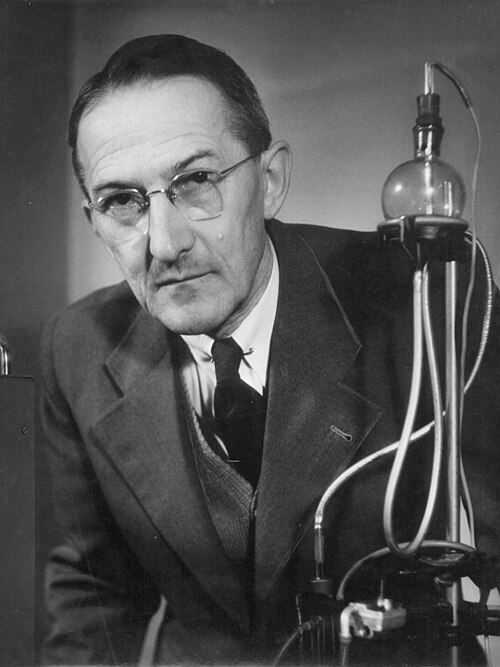
\includegraphics[width=\linewidth]{images/book3/heyrovsky.jpg}
\end{minipage}\hfill
\begin{minipage}[t]{0.71\linewidth}
\vspace{0pt}
1922 年，雅罗斯拉夫·海洛夫斯基记录了通过一根汞电极的电流，
该汞电极在毛细管尖端一滴接一滴地形成汞滴，同时电势被连续扫描：
每种可还原的物种给出一个台阶，台阶的位置可用来鉴别它，
其高度则度量其浓度。不断更新的汞滴使表面
保持新鲜，而氢在汞上的高过电势开辟了一个很宽的
阴极窗口。极谱法为他赢得了 1959 年的诺贝尔化学奖，
并奠定了电分析化学的基础；照片中他手持一支
滴汞电极。（照片来源：J. 海洛夫斯基物理化学研究所档案，
CC BY-SA 3.0，维基共享资源。）
\end{minipage}
\end{history}

\section{练习}

\begin{exercise}[$\star$]\label{exo:b2:current-potential-curves:1}
在输出电流的丹尼尔电池中，
按本章约定，给出锌电极和铜电极处
电流的符号。
\end{exercise}

\begin{exercise}[$\star$]\label{exo:b2:current-potential-curves:2}
计算 \ce{Ag+} 还原的极限电流（\qty{2.0}{mmol/L}，$D =
\qty{1.6e-9}{m^2/s}$），电极面积 \qty{0.50}{cm^2}，取 $\delta = \qty{25}{\micro m}$
（模型数值）。
\end{exercise}

\begin{exercise}[$\star$]\label{exo:b2:current-potential-curves:3}
依本章的模型曲线，如何辨认一个快速体系与
一个慢速体系？各举一例，均以铂为电极。
\end{exercise}

\begin{exercise}[$\star$]\label{exo:b2:current-potential-curves:4}
某溶液仅含 \ce{Fe^2+}。其阳极电流
达到平台一半时的电势为何（设两种形式扩散速率相同，$E^\circ = \qty{0.77}{V}$）？
\end{exercise}

\begin{exercise}[$\star\star$]\label{exo:b2:current-potential-curves:5}
铂电极浸于 \ce{Fe^3+} 与 \ce{Cu^2+} 的溶液中（两者浓度相等，
$E^\circ$ 分别为 0.77 与 \qty{0.34}{V}），向负电势方向扫描。
请描述该曲线：各波、平台、它们的高度，以及
阴极壁垒。
\end{exercise}

\begin{exercise}[$\star\star$]\label{exo:b2:current-potential-curves:6}
在\cref{exo:b2:current-potential-curves:5}的溶液中，电极的电势
先保持在 \qty{0.50}{V}，再保持在 \qty{0.10}{V}，
两种情况下各发生什么？
\end{exercise}

\begin{exercise}[$\star\star$]\label{exo:b2:current-potential-curves:7}
求水在 pH 为 0 和 pH 为 14 时两个电对的能斯特电势，并
画出铂上电活性窗口随 pH 移动的示意图。
\end{exercise}

\begin{exercise}[$\star\star$]\label{exo:b2:current-potential-curves:8}
\ce{Fe^2+} 被 \ce{Ce^4+} 滴定，同时铂电极保持在
\qty{1.0}{V}，记录电流。画出电流随所加体积的变化示意图，
并说明它如何确定化学计量点（\ce{Ce^4+}/\ce{Ce^3+}：$E^\circ =
\qty{1.72}{V}$）。
\end{exercise}

\begin{exercise}[$\star\star$]\label{exo:b2:current-potential-curves:9}
将搅拌速率加倍，则扩散层厚度减半。
对于快速体系，平台、半波电势以及零电流
电势各会发生怎样的变化？
\end{exercise}

\begin{exercise}[$\star\star\star$]\label{exo:b2:current-potential-curves:10}
推导仅含还原态 Red 的快速体系的波方程，并
证明以 $E$ 对 $\log[i/(i_{\lim} - i)]$ 作图得一直线，
其斜率在 \qty{25}{\degreeCelsius} 时为 $0.059/n$ 伏特。
\end{exercise}

\begin{exercise}[$\star\star\star$]\label{exo:b2:current-potential-curves:11}
一块锌片浸入 \qty{1}{mol/L} 的酸中，溶解得很慢；
而与铂丝接触的同一块锌片溶解得很快，铂丝上有氢气冒出。
试用电流–电势曲线加以解释。
\end{exercise}

\begin{exercise}[$\star\star\star$]\label{exo:b2:current-potential-curves:12}
要氧化 pH 为 0 时波位于 \qty{2.0}{V} 的某物种，
应选铂电极，还是选氧过电势高的电极？
请说明理由，并说明否则会生成什么。
\end{exercise}

\section{问题：河流的氧探针}

\begin{problem}[{周末问题——安培型氧传感器的阴极、
通过其膜的极限电流、用亨利定律在空气饱和水中的标定，
以及河流中的氧含量}]
\label{pb:b2:current-potential-curves:1}
一根安培型氧探针以金为阴极、银为阳极，二者浸于
氯化钾凝胶中，并通过一层薄的透气膜与样品隔开。
阴极保持在 \qty{-0.60}{V}（相对于银–氯化银阳极）。
\qty{25}{\degreeCelsius} 时的数据：\ce{O2} 的亨利定律常数
$H = \qty{1.3e-5}{mol/(m^3.Pa)}$；水的蒸气压
\qty{3.17}{kPa}；干燥空气中氧的体积分数为 20.95~\%；$E^\circ(\ce{O2}/\ce{H2O}) =
\qty{1.229}{V}$；$E^\circ(\ce{AgCl}/\ce{Ag}) = \qty{0.222}{V}$。膜（模型值）：
面积 \qty{0.10}{cm^2}，厚度 \qty{25}{\micro m}，
\ce{O2} 穿过膜的有效扩散系数 \qty{1.0e-10}{m^2/s}。
% ledger: henry:O2, pvap:H2O.298, air:O2, dfg:Cl-_ao, dfg:AgCl_cr, aw:O

\medskip
\noindent\textbf{第一部分——阴极。}
\begin{enumerate}
  \item 写出中性介质中氧气的还原反应。
  \item 写出银阳极上的反应，以及总反应。
  \item 计算 \ce{O2}/\ce{H2O} 电对在 pH 为 7 时的能斯特电势，
        取 $p_{\ce{O2}} = \qty{0.21}{bar}$。
  \item 将阴极电势（相对于 Ag/AgCl 为 \qty{-0.60}{V}）换算到
        氢标，取凝胶中氯离子的活度为 1。
  \item 为什么阴极必须保持得远低于
        \ce{O2} 的能斯特电势？
  \item 为什么选择平台上的电势？
  \item 可用电势的下限由什么决定？
\end{enumerate}

\medskip
\noindent\textbf{第二部分——极限电流。}
\begin{enumerate}[resume]
  \item 阴极工作在平台上时，描述 \ce{O2} 穿过膜的
        浓度分布。
  \item 写出 \ce{O2} 通过膜的通量。
  \item 推出电流与溶解的
        \ce{O2} 浓度 $c$ 的函数关系。
  \item 为什么用膜的厚度代替扩散层厚度？
  \item 为什么读数几乎与河流的搅拌无关，却
        极大地依赖于膜的污染？
\end{enumerate}

\medskip
\noindent\textbf{第三部分——标定。}
\begin{enumerate}[resume]
  \item 计算与空气饱和的水上方 \ce{O2} 的分压，
        在 \qty{1.013}{bar}、\qty{25}{\degreeCelsius} 下。
  \item 计算饱和时溶解 \ce{O2} 的浓度，
        单位为 \unit{mol/m^3}。
  \item 将其换算为 \unit{mg/L}。
  \item 预测探针在空气饱和水中的电流。
  \item 探针在空气饱和水中的实际读数为 \qty{4.05}{\micro A}
        （练习数据）。计算其灵敏度，单位为 \unit{\micro A} 每
        \unit{mg/L}。
  \item 为什么要标定，而不直接相信预测的电流？
  \item 在除去氧的水中，探针应读出多少？
\end{enumerate}

\medskip
\noindent\textbf{第四部分——河流。}
\begin{enumerate}[resume]
  \item 在 \qty{25}{\degreeCelsius} 的一份河水样品中，探针读数为
        \qty{2.80}{\micro A}。计算溶解氧的浓度，单位为 \unit{mg/L}。
  \item 将其表示为饱和百分比。
  \item 河流源头的水几乎被氧饱和，
        请给出溶解氧亏缺的一个原因。
  \item 探针在一小时内消耗的 \ce{O2} 的物质的量是多少？
        这会干扰样品吗？
  \item 若河水温度为
        \qty{15}{\degreeCelsius}，为什么必须重新标定？
  \item 给出样品中溶解氧的浓度。
\end{enumerate}
\end{problem}
